\documentclass[10pt,oneside,a4paper]{article}
\usepackage[utf8]{inputenc}
\usepackage{amsmath}
\usepackage{indentfirst}
\usepackage{enumitem}
\usepackage[spanish]{babel}
\usepackage[export]{adjustbox}
\usepackage{graphicx}
\graphicspath{ {img/} }
\usepackage{listings}
\usepackage{subfig}
\usepackage{cite}

\addtolength{\oddsidemargin}{-.300in}
\addtolength{\evensidemargin}{-.300in}
\addtolength{\textwidth}{0.600in}
\addtolength{\topmargin}{-.300in}
\addtolength{\textheight}{0.600in} %1.75

\begin{document}
\begin{titlepage}

\title{\Huge Rendering Avanzado  \\[0.7in] \LARGE \textit{Path Tracing}\\[3.6in]}
\date{}
\author{Álvaro Muñoz Fernández\\
Iván Velasco González}
\maketitle
\thispagestyle{empty}
\end{titlepage}

\section{Path Tracing}
En esta parte de la práctica se debían implementar varios algoritmos de \textit{ Path Tracing} que se verán mas adelante es subsiguientes secciones.
\subsection{Naive Path Tracing}
En esta sección se pedía implementar un método de \textit{Path Tracing} básico, teniendo en cuenta unicamente la BRDF de los materiales. Por lo tanto, este es muy similar al realizado en la practica anterior (\textit{direct\_mats}) , con la salvedad de que, no se limitara la profundidad del camino a un único rayo, sino que podrán tener mas profundidad, consiguiendo mas rebotes por la escena, y por tanto, iluminación global.\\

Debido a las similitudes con el \textit{direct\_mats}, se decidió utilizar este como base. En primer lugar, se añadieron una serie de variables como: \textit{L}, la cual almacena la iluminación total calculada para un punto en concreto, la cual se inicializa a 0; \textit{W} la cual almacena todos los multiplicadores, como la brdf, pdfs, etc.. que se irán acumulando tras los sucesivos rebotes, la cual se inicializa a 1, y por ultimo, una variable que representa el rayo que se esta tratando, \textit{mRay}, la cual se inicializa con el primer rayo trazado desde la cámara.\\

Seguidamente, se ha implementado un bucle infinito que se encargara de computar la iluminación en si. En primer lugar, se comprueba si el rayo que se esta trazando en ese momento interseca con la geometría de la escena, si esto no es así se suma a la iluminación total del punto, la iluminación proporcionada por el ambiente multiplicada por todas las interacciones de la luz (\textit{W}) y se devuelve la iluminación total calculada. En el caso de que el rayo si interseque con geometría de la escena, se comprueba si ha intersecado con una fuente de luz, si esto es así se suma a la iluminación total en el punto la iluminación de esa fuente de luz multiplicada por \textit{W}. Seguidamente, se comprueba si se debe de seguir trazando rayos por el método de ruleta rusa, se comprueba si un numero aleatorio, distinto que los utilizados para samplear, es menor que la probabilidad de que continué el rayo, si esto es así, se sale del bucle de iluminación y se devuelve la iluminación calculada hasta el momento. En caso de que se deba de seguir trazando rayos, se samplea la BRDF del  material con el que se ha intersecado, y se calcula el nuevo rayo a utilizar (\textit{mRay}). Ademas, se actualiza el valor de \textit{W} con las características de este nuevo rebote de la siguiente forma:
$$W *= \frac{brdf * cos\theta}{pdf_{dir} * pdf_{surv}}$$

Donde $\theta$ es el angulo entre la normal del punto a tratar y el angulo de salida del rayo, y $pdf_{surv}$ es la probabilidad de supervivencia de un rebote, este ultimo termino es necesario añadirlo debido a la utilización del método de ruleta rusa para terminar con los rebotes de la luz.

\begin{figure}[h]
\centering
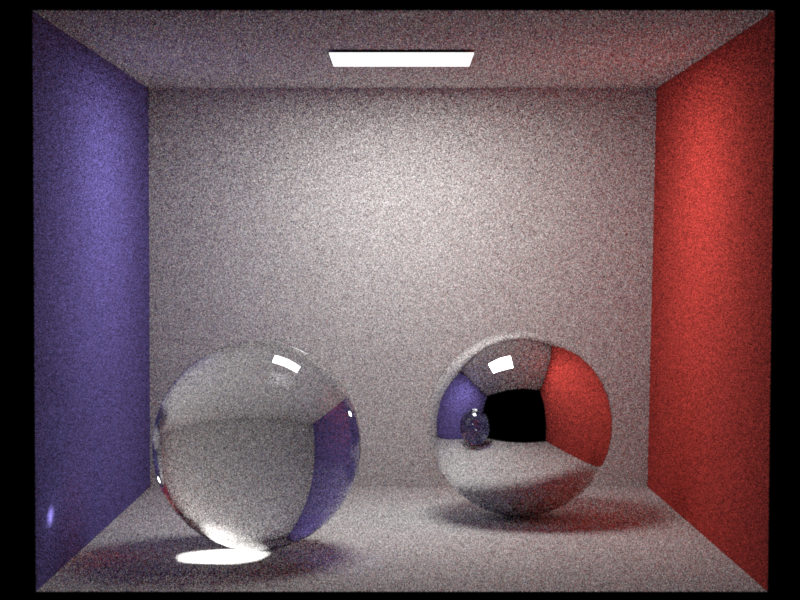
\includegraphics[width=.6\linewidth]{images/cbox_path_512.png}
\caption{Imagen generada utilizando \textit{Path Tracing} simple}
\label{fig:disp}
\end{figure}

Como puede verse en la imagen, se han conseguido varios efectos de iluminación global, como los reflejos en la esfera de espejo o la caustica en la esfera que representa un cristal, ademas de un poco de \textit{ color bleding} en el techo proveniente de las paredes. Sin embargo, se aprecia una gran cantidad de ruido tanto en las paredes, como en los reflejos. Ademas, el dieléctrico aunque se puede observar que la luz puede pasar a través de el, se ve prácticamente negro debido a la dificultad de encontrar un camino que lo atraviese y llegue a una fuente de luz, mientras que la caustica si que tiene una apariencia aceptable.\\

Por otro lado, la convergencia de la imagen no es muy buena debido a que solamente los caminos que intersequen con una fuente de luz contribuirán a la iluminación final. Por lo tanto, una gran cantidad de muestras se desperdician al no encontrar la luz.

\subsection{Path Tracing with Next-Event Estimation}
En esta parte de la práctica se va a implementar un \textit{Path tracer} algo mas sofisticado que resuelva algunos de los problemas de la versión anterior. En concreto, trata de resolver el problema de convergencia que provocan los caminos que no intersecan con ninguna luz, y que por tanto, no aportan nada a la escena. Para resolver esto, se va a calcular en cada rebote, la iluminación directa que recibe ese punto desde una fuente de luz, con esto se consigue que cada rebote tenga, en la mayoría de los casos, algo de aporte de luz garantizando haciendo que todos los rebotes contribuyan a la iluminación , lo que mejora la convergencia. Ademas, se siguen trazando los rayos impuestos por la BRDF para conservar la iluminación global.\\

Para realizar esta tarea se ha partido del código implementado en la sección anterior, pero se ha añadido un nuevo bloque de código que, para cada rebote \textit{samplea} una fuente de luz aleatoria y calcula su aportación a la luz del punto a tratar como:
$$ L += \frac{Li * brdf_{nee} * V * W}{pdf_{dir} * pdf_{light}}$$

Donde: $Li$ es la iluminación directa que llega al punto desde la fuente de luz sampleada; $brdf_{nee}$ es el termino brdf teniendo en cuenta la dirección del rayo de entrada, y al dirección del rayo de salida, el que va hacia la luz; $V$ es el termino de visibilidad, ya que, como hemos sampleado al luz esta podría estar ocluida y , por ultimo $pdf_{light}$ y $pdf_{dir}$ son las pdf de la luz sampleada y del punto en concreto sampleado respectivamente. \\

Ademas, hay que tener en cuenta que al incluir un rayo directo a la luz puede darse el caso de que para un mismo punto se sume la aportación de una fuente de luz dos veces, una al samplear esa fuente de luz y la otra si el rayo de la brdf interca con esa misma fuente de luz. Para evitar estos casos se ha añadido un \textit{flag} que indica si se debe contar la iluminación si la brdf cae en una fuente de luz o no, mientras que la aportación de \textit{Nee} siempre se tiene en cuenta. Debiendo contar con la iluminación de la brdf si: es el primer rebote, para evitar que las fuentes de luz se vean negras; y si el material es completamente especula, es decir de tipo \textit{EDISCRETE}, ya que este tipo de materiales no pueden samplearse utilizando iluminación directa (tanto su brdf como pdf devuelven siempre 0).\\

\begin{figure}[h]
\centering
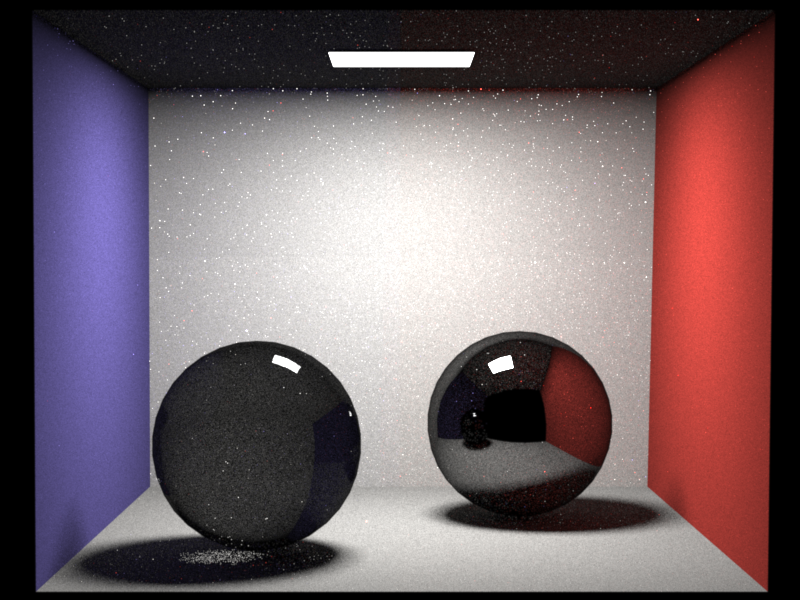
\includegraphics[width=.6\linewidth]{images/cbox_pathNee_512.png}
\caption{Imagen generada utilizando \textit{Path Tracing} con \textit{Nee}}
\label{fig:disp}
\end{figure}

Como puede observarse en la imagen, se ha conseguido el resultado esperado obteniendo muchísima mejor convergencia a igual numero de muestras para esta escena, donde ha mejorado tanto la iluminación de las paredes como los reflejos y sobre todo el interior del dielectrico que ya no es tan negro. Sin embargo, sigue habiendo problemas con las causticas, las cuales tiene mucho ruido, y ademas, ahora se puede apreciar el ruido introducido por los rebotes especulares y la refracción del dielectrico como puntos de mucha mayor intensidad que el resto en la pared trasera.
 
 \subsection{Interesting Image}
En esta imagen de ejemplo, se pueden observar la gran mayoría de efectos que se peuden conseguir utilizando \textit{ Path Tracing} con \textit{Next-Event Estimation} utilizando nuestra implementación.

\begin{figure}[h]
\centering
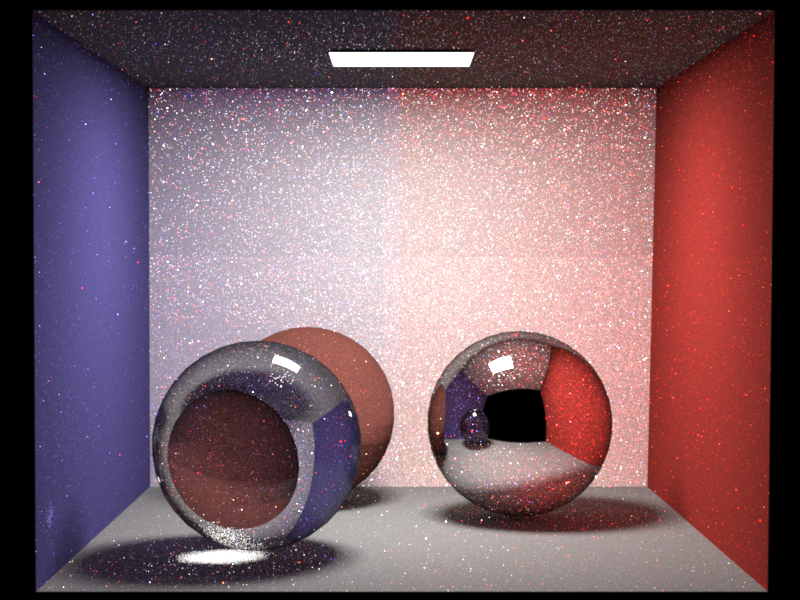
\includegraphics[width=.6\linewidth]{images/cbox_interesting_nee_512.png}
\caption{Imagen generada utilizando \textit{Path Tracing} con \textit{Nee} y un valor bajo de absorción}
\label{fig:disp}
\end{figure}

Para la generación de esta imagen se ha utilizado un nivel mas bajo de absorción (modelado por la probabilidad de sobrevivir a la ruleta rusa), para conseguir que la esfera del dielectrico se viera mas clara y ademas la caustica fuese mas acentuada. Sin embargo, al bajar la absorción nos encontramos con un exceso de \textit{color bleeding} en la pared del fondo. Esto es debido a que en nuestra implementación se utiliza la misma probabilidad de sobrevivir a un rebote para todos los materiales de la escena. Sin embargo, esto en la realidad no es así y cada material tienen un nivel de absorción distinto. Por ejemplo, el nivel de absorción del cristal seria muy inferior al de las paredes, y por tanto si obtuviésemos la probabilidad de sobrevivir a un rebote del material en cuestión , en lugar de una constante global, se podrían conseguir escenas mas realistas, pudiendo eliminar el \textit{color bleeding}, sin oscurecer las esferas.   
  

\end{document}